
\documentclass[11pt,a4paper]{article}
\usepackage[utf8]{inputenc}
\usepackage{amsmath}
\usepackage{amsfonts}
\usepackage{amssymb}

\usepackage[table]{xcolor}

\usepackage{graphicx}
\usepackage{float}

\usepackage[german]{babel}

\usepackage[backend=biber,citestyle=authoryear-comp]{biblatex}

\addbibresource{Sources.bib}

\usepackage[left=3cm, right=3cm, top=3cm, bottom=3cm]{geometry}
\numberwithin{equation}{subsection}

\author{David Bailey}
\title{AML Protokol Optomechatronik}

\linespread{1.1}

\begin{document}
\selectlanguage{german}

\begin{titlepage}
	\centering
	{Leibniz Universität Hannover\par}
	{\large Kleine Laborarbeit\par}	

	\vspace{4.5cm}	
	
	{\huge \bf AML Optomechatronik \par}
	{\Huge \bf Spektralanalyse eines LCD-Beamers\par}
	\vspace{0.3cm}
	
	\vspace{1.5cm}
	
	{\Large David Bailey 	\\
			Simon Hecht		\\
			Lukas Held		\\
			Anis Ferjani	\\
			Albert Nessa	\\
			Mohamed Raafat Nciri \par}

	\vfill

	\raggedright

{\Large
\begin{tabular}{ll}
Gruppennummer:& 25 \\
Versuch durchgeführt:& 07.11.2019 \\
Abgabe des Berichtes:& 14.11.2019 \\
Anzahl der Seiten:& 13
\end{tabular}\par}

\end{titlepage}

\tableofcontents
\newpage

\section{Einführung}

Die Optomechatronik ist ein sehr modernes und weitreichendes Forschungsgebiet. Die Anwendung optomechatronischer Systeme spannt sich von simpler Beleuchtung über Projektion und Informationsübertragung bis hin zu optischen Bearbeitungsverfahren für Mikro- und Nanostrukturen. ``Optomechatronik'' steht hierbei für die Kombination aus Optik, Informatik, Elektronik und Mechanik. Ingenieure welche sich mit diesen Technologien befassen müssen also ein breites Feld an Technologien beherrschen.

Der Versuch ``Kleine Laborarbeit Optomechatronik'' soll den Teilnehmenden einen ersten Einblick in dieses Themengebiet ermöglichen, und ihnen wichtige Grundlagen zur Verwendung und Analyse optomechatronischer Systeme vermitteln. Als Beispiel wird hierfür ein handelsüblicher LCD-Beamer verwendet, dessen einzelne Bestandteile von den Teilnehmenden separat mit optischen Messverfahren untersucht werden. Auch wichtig ist hierbei die Betrachtung der menschlichen Farbwahrnehmung, und wie der Beamer für Zuschauende ein nahezu durchgängiges Farbspektrum generieren kann.

Zusätlich werden alternative Technologien wie z.B. der One-Chip-DLP Beamer angesprochen, und es werden die Messverfahren selbst genauer erklärt, um den Teilnehmenden ein eigenständiges Ausführen, Auswerten und Korrigieren der folgenden Versuche zu ermöglichen.



\newpage

\section{Versuchsteile}
\subsection{Teilversuch 1 - Transmissionsanalyse}

Der erste Teilversuch befasst sich mit sogenannten dichroitischen Spiegeln. Diese sind dünne Platten, welche in der Optomechatronik zur Aufspaltung farbigen Lichtes dienen. Erreicht wird dies durch Dünnfilminterferenz, welche bestimmte Wellenlängen reflektiert bzw. unbeeinflusst durch den Spiegel passieren lässt. Für den später betrachteten LCD-Beamer liefen diese Spiegel die verschiedenen Farben, und sind so integraler Bestandteil dessen Farbwiedergabe.

Es sollen zwei dieser Spiegel von den Teilnehmenden mithilfe eines Spektrometers untersucht werden, um deren Transmissionsspektren zu messen. Darauf folgend können die Reflektionsspektren der Spiegel bestimmt werden, um somit die Farbpositionen der reflektierten Lichtstrahlen im Farbdreieck zu bestimmen.

\subsubsection{Versuchsaufbau} Dieser besteht aus einer möglichst weißen, spektral verteilten Lichtquelle, hier einer LED mit Photphor. Das Licht der LED wird mithilfe eines Spiegels zu einem Strahl gebündelt, welcher auf die Messapertur eines Spektrometers gerichtet wird. Das Spektrometer ist von einem Computer aus bedienbar, und es können die gemessenen Spektren gespeichert werden. Zusätzlich steht den Teilnehmenden eine Halterung zur Verfügung, mit derer sich die dichroitischen Spiegel in den Lichtstrahl der LED, vor dem Spektrometer, in einem $45^\circ$-Winkel relativ zum Lichtstrahl befestigen lassen. Das reflektierte Licht wird auf eine weiße Abschirmung geworfen, um sichtbar gemacht zu werden.

\begin{figure}[h]
	\centering
	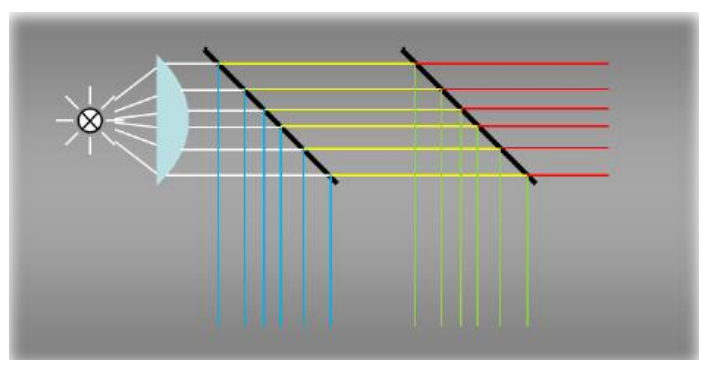
\includegraphics[scale=0.4]{Images/Aufbau.png}
	\caption{Schematischer Versuchsaufbau, [\cite[Abb. 3.2]{AML_SKRIPT}]}
\end{figure}

\subsubsection{Versuchsdurchführung}

Die Messung der Transmissionsspektren der Spiegel erfolgt in vier Schritten:
\begin{itemize}
\item Bestimmung einer Integrationszeit, bei welcher das Spektrometer zu ca. 75\% belichtet wird. Hierdurch wird eine Überbelichtung und somit Verfälschung der Messergebnisse verhindert. Im folgenden wird eine Integrationszeit von 90ms gewählt.
\item Durchführung einer Dunkelmessung des Hintergrundlichtes, um dieses aus den Messwerten entfernen zu können.
\item Durchführung einer Referenzmessung (100\%-Messung) der LED ohne eingebaute Spiegel. Mit dieser werden die späteren Messwerte automatisch normiert, um somit die relativen Anteile des transmittierten Lichtes berechnen zu können.
\item Messung der relativen Spektren von jeweils Spiegel 1 und Spiegel 1+2
\end{itemize}
In der folgenden Grafik sind die drei relevanten Kurven der relativen Spektren von Referenzmessung, von Spiegel 1 und von Spiegel 1+2 im sichtbaren Frequenzbereich dargestellt:

\begin{figure}[h]
	\centering
	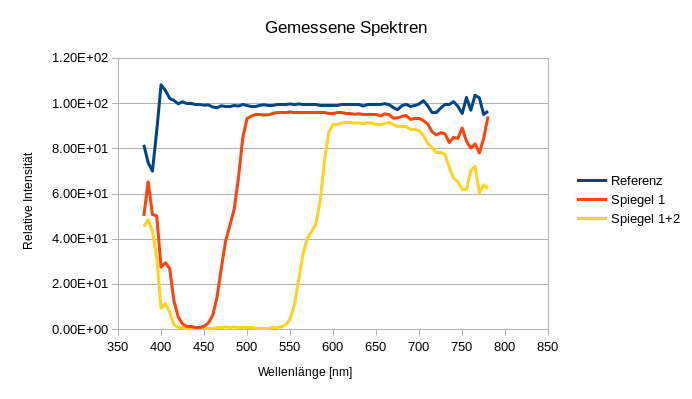
\includegraphics[scale=0.8]{Images/V1_Spektren.png}
	\caption{Relative Spektren der Spiegel im Vergleich}
	\label{V1_RES}
\end{figure}

\subsubsection{Auswertung}

Zuerst wird die Kurve der Referenzmessung betrachtet. Überwiegend liegt diese bei 100\%, wie es von der Referenzmessung zu erwarten ist. An der oberen und unteren Grenze des für den menschlich sichtbaren Wellenlängenbereiches kommt es jedoch zu Schwankungen. Diese lassen sich dadurch erklären, dass die verwendete LED in diesen Wellenlängen sehr schwach bis nicht leuchtet, und die Messwerte hierdurch stark vom Hintergrundrauschen beeinflusst werden. 

Das Spektrum des ersten Spiegels in Abb. \ref{V1_RES} lässt nun auf zweierlei schließen:
Die Transmission des Spiegels ist nicht vollständig, es wird anscheinen immer ein kleiner Teil des Lichtes reflektiert bzw. absorbiert. Erkennbar ist dies daran, dass die Kurve nie ganz 100\% erreicht. Zweitens ist deutlich der Bereich der Reflekion zwischen 400nm und 500nm zu erkennen, in welchem der Spiegel fast 100\% des Lichtes reflektiert. 

Schließlich wird das Spektrum beider Spiegel (1+2) betrachtet. Erstens ist zu erkennen dass es im Vergleich zu Spiegel 1 eine stärkere allgemeine Reflektion bzw. Absorption auch in nicht-reflektierten Wellenlängen gibt. Zweitens ist zu erkennen dass der zweite Spiegel einen Wellenlängenbereich von ca. 450nm bis 600nm reflektiert, da dort keines des vom Spiegel 1 durchgelassenen Lichtes mehr am Sensor an kommt.

Nun werden die jeweiligen relativen reflektierten Spektren der Spiegel ermittelt. Unter der Annahme dass das nicht tranmittierte Licht zu 100\% reflektiert wird, wird vom bekannten Referenzspektrum das Transmissionsspektrum des ersten Spiegels, bzw. vom Transmissionsspektrum des ersten Spiegels das Transmissionsspektrum des ersten und zweiten Spiegels abgezogen, und nach ersterem Spektrum normiert.

\begin{eqnarray}
	R_{1, \lambda}(\lambda) = & \frac{D_{\lambda,0}(\lambda) - D_{\lambda,1}(\lambda)}{D_{\lambda,0(\lambda)}} \\
	R_{2, \lambda}(\lambda) = & \frac{D_{\lambda,1}(\lambda) - D_{\lambda,1+2}(\lambda)}{D_{\lambda,1}(\lambda)}
\end{eqnarray}
Es ergeben sich folgende Kurven:

\begin{figure}[h]
	\centering
	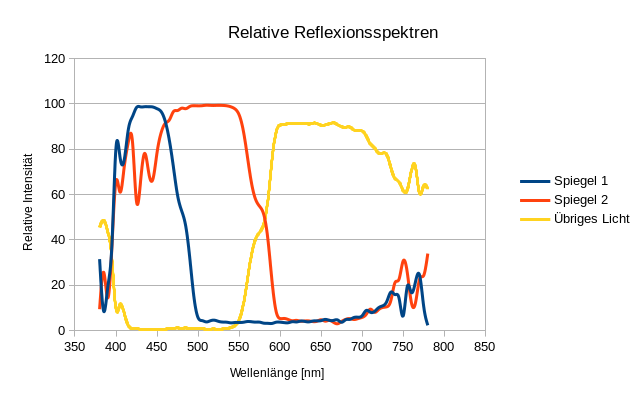
\includegraphics[scale=0.8]{Images/V1_Reflexionsspektren.png}
	\caption{Berechnete relative Reflektionsspektren der zwei Spiegel plus übriges transmittiertes Licht}
	\label{V1_REFLECT}
\end{figure}

Die vorher vermuteten Reflektionsbereiche von 400nm bis 500nm bzw. 450nm bis 600nm sind hier gut erkennbar. Die starken Schwankungen des Reflektionsspektrums des zweiten Spiegels unter 450nm lassen sich durch niedrige absolute Werte erklären, welche somit stärker rauschen.
Das Verhalten der Spiegel kann somit als Bandpassfilter angenähert werden, welche für die obig genannten Wellenlängenbereiche das Licht reflektieren, ansonsten beinahe ungestört transmittieren.

\newpage
\subsection{Teilversuch 2 - Lichstrommessung}
Der zweite Teilversuch befasst sich mit der Lichtquelle eines handelsüblichen LCD-Beamer, einer sogenannten Quecksilberdampflampe. Sie liefert durch Gasentladungen einen starken, gebündelten und möglichst gleichmäßig spektral verteilten Lichtstrahl, welcher zur Projektion der Bilder des Beamers verwendet wird. Das Spektrum dieser Lampe beeinflusst maßgeblich die Farben, welche dem später betrachteten LCD-Beamer zur Verfügung stehen, und ist somit in Kombination mit den dichroitischen Spiegeln wichtiger Teil der Farbwiedergabe selbst.

In diesem Versuch soll das Spektrum und der Lichtstrom $\Phi_{e,\lambda}$ einer solchen Quecksilberdampflampe mithilfe einer Ulbrichtkugel bestimmt werden. Wichtig ist hierbei auch eine korrekte Vermessung eines Referenz- und Absorptionsspektrums, um aus dem gemessenen Spektrum der Lampe auf den realen Lichtstrom schließen zu können.

\subsubsection{Versuchsaufbau}

Der Versuchsaufbau besteht aus einer bereits aufgebauten Ulbrichtkugel inklusive Spektrometer, der Quecksilberdampflampe und einer Absorptionskorrekturlampe. Um die Lampen betreiben zu können steht eine Spannungsquelle zur Verfügung. Das Spektrometer wird von einem Computer aus bedient, von welchem die gemessenen Spektren gespeichert werden können.

\subsubsection{Versuchsdurchführung}

Die Kalibrationsdaten der im Versuch verwendeten Ulbrichtkugel sind bekannt. Für andere, nicht bereits kalibierte Kugeln muss vor dem Versuch noch das Referenzspektrum $D_{\lambda,ref}$ einer bekannten Referenzlampe (mit $\Phi_{e\lambda,ref}$), sowie das Spektrum der Absorptionskorrekturlampe $K_{\lambda,ref}$ (ohne eingebaute Quecksilberdampflampe) bestimmt werden.

Die Messung des Spektrums der Quecksilberdampflampe ($D_\lambda(\lambda)$) erfolgt in den folgenden Schritten:

\begin{itemize}
\item Das Spektrum der Absorptionskorrekturlampe mit eingebauter Quecksilberdampflampe, $K_\lambda$, wird gemessen. Die Absorptionskorrekturlampe wird hierfür eingeschaltet, die Dampflampe bleibt aus. Das Spektrum wird am Computer gespeichert.
\item Das Spektrum der eingeschalteten Quecksilberdampflampe, $D_\lambda$, wird gemessen. Hierfür muss die Lampe einige Minuten vorwärmen, um sich zu stabilisieren. Der Lüfter der Lampe muss hierfür laufen, da sich die Lampe ansonsten zu stark erhitzt. Das Spektrum wird am Computer abgespeichert.
\end{itemize}
Die gemessenen Spektren sind in Grafiken \ref{V2_AKL} und \ref{V2_QDL} dargestellt.

\subsubsection{Auswertung}

\begin{figure}[h]
	\centering
	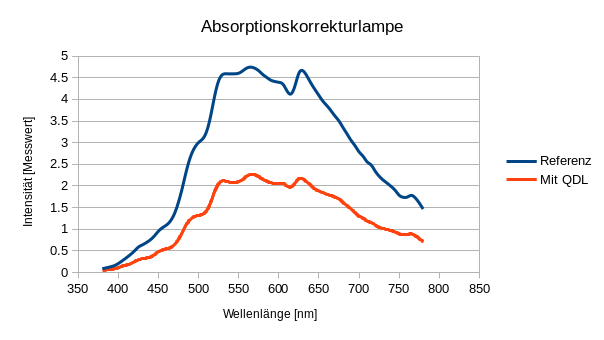
\includegraphics[scale=0.8]{Images/V2_AKL.png}
	\caption{Gemessenes Spektrum der Absorptionskorrekturlampe im Vergleich zum Referenzspektrum}
	\label{V2_AKL}
\end{figure}

Zuerst wird das Absorptionsspektrum der Absorptionskorrekturlampe, sichtbar in Abbildung \ref{V2_AKL}, mit dem bereitgestellten Referenzwert verglichen. Deutlich zu sehen ist, dass der gemessene Wert um einen Faktor von etwa 2 kleiner ist als der Referenzwert. Das Gehäuse der Quecksilberdampflampe absorbiert also etwa die Hälfte des Lichtes, gleichmäßig über das Spektrum verteilt.
Zur Berechnung der Korrekturfaktoren muss lediglich das Referenzspektrum durch das gemessene Spektrum dividiert werden.
\begin{equation}
\frac{K_{\lambda,ref}(\lambda)}{K_{\lambda}(\lambda)}
\end{equation}

\begin{figure}[h]
	\centering
	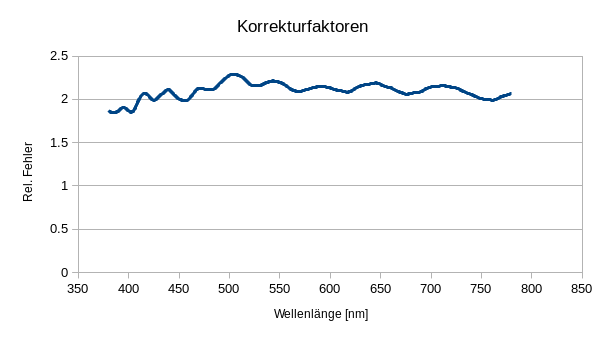
\includegraphics[scale=0.7]{Images/V2_Korr.png}
	\caption{Berechnete Wellenlängenabhängige Korrekturfaktoren}
	\label{V2_KOR}
\end{figure}

\begin{figure}[h]
	\centering
	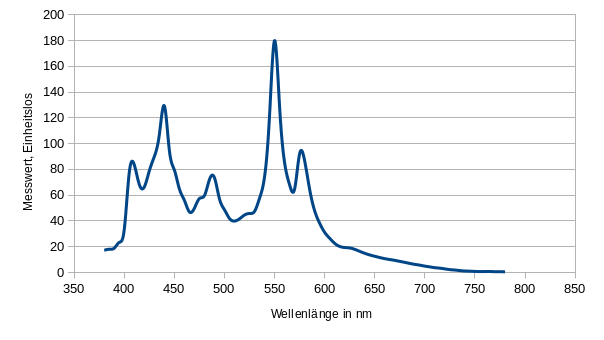
\includegraphics[scale=0.7]{Images/V2_Dampflampe.png}
	\caption{Messwerte des Quecksilberdampflampenspektrums}
	\label{V2_QDL}
\end{figure}

In Abbildung \ref{V2_KOR} ist deutlich ein einheitlicher Faktor von ca. 2 erkennbar, welcher nur leicht mit der Wellenlänge schwankt. Dies ist vom schwarzen Plastikgehäuse zu erwarten.


\newpage
\subsection{Teilversuch 3 - Reale Farbpunktbestimmung}

In den ersten zwei Teilversuchen wurden die für die Farbgebung eines Beamers wichtigen Bauteile untersucht. Der dritte Teilversuch befasst sich nun mit der Analyse eines vollständigen Beamers und dessen Farbwiedergabe, um reale Werte für den Vergleich mit den berechneten Erwartungswerten zu liefern.

Mithilfe eines Goniometers und einer Leuchtdichtekamera werden die drei Farbkomponenten des Beamers über dessen Projektionsfläche gemittelt berechnet, um den Teilnehmenden eine Berechnung des realen Farbraumes zu ermöglichen.

\subsubsection{Versuchsaufbau}

Der Aufbau besteht aus einem Goniometer, d.h. einer automatisch drehbaren Platform, auf welche der Beamer befestigt ist. Der Beamer ist auf eine Leuchtdichtekamera gerichtet, welche mithilfe verschiedener Filter die Rot-, Grün- und Blauanteile des vom Beamer ausgestrahlten Lichtes misst. Ein Computer wird verwendet, um die Spektren der Leuchtdichtekamera zu speichern und um den Beamer und das Goniometer anzusteuern.

\subsubsection{Versuchsdurchführung}

Die Messung der drei Farbkomponenten wird in den folgenden Schritten durchgeführt:
\begin{itemize}
\item Die Belichtungszeit der Leuchtdichtekamera wird für die drei Farben so bestimmt, dass nicht im Sättigungsbereich des Sensors gemessen wird. Für die Teilnehmenden wurden bereits bestimmte Werte für die drei Farben vorgegeben.
\item Es werden 15 Rotationen des Goniometer, welche möglichst gleichmäßig über die Projektionsfläche des Beamers verteilt sind, ausgewählt. Die Teilnehmenden wählten Winkel von $+15^\circ$; $\pm2.5^\circ$ aus.
\item Es wird ein PDF einer der drei Farben (Rot, Grün oder Blau) über den Beamer projiziert, und für die gewählte Farbe über die 15 Goniometerrotationen gemittelt der Farbpunkt gemessen. Der berechnete Farbpunkt wird abgespeichert, und dieser Schritt wird für alle drei Farben ausgeführt.
\end{itemize}

Zu beachten ist, dass das PDF mit den Farbbildern nicht unbedingt 100\% die Farbkanäle des Beamers ansteuert. Es gibt so z.B. immer eine gewisse Farbraumumrechnung, welche die Messwerte der Farbpositionen beeinträchtigen kann. Quantifizert werden kann dies unter Kenntnis des für das PDF verwendeten Farbraums, des Farbraumes des Beamers selbst, sowie eventueller Kalibrationsparameter des Beamers, die hier durch fehlende Spezifikation nicht genauer betrachtet werden können. Auch wird die Standardabweichung der einzelnen Farbwerte berechnet, um die Varianz der Farben quantifizieren zu können. Der gemessene durchschnittliche Farbraum, berechnet nach [\cite[Seite 27]{AML_SKRIPT}], ist in Tabelle \ref{tab:TV3_Averages} sowie in der Auswertung in Abschnitt \ref{A_FCOORDS} zu sehen.

\begin{eqnarray*}
x_{n,m} = &\frac{1}{N}\sum_{k=1}^{N} x_{n,k} \\
y_{n,m} = &\frac{1}{N}\sum_{k=1}^{N} y_{n,k} \\
x_{n,\sigma} = &\sqrt{\frac{1}{N-1}\sum_{i=1}^{N}\left(x_{n,i}-x_{n,m}\right)}  \\
y_{n,\sigma} = &\sqrt{\frac{1}{N-1}\sum_{i=1}^{N}\left(y_{n,i}-y_{n,m}\right)}
\end{eqnarray*}

\begin{table}[h!]
\centering
\caption{Statistische Werte der Farbraummessung}
\label{tab:TV3_Averages}
\begin{tabular}{| c | c | c | c | c |}
\hline
n & $x_{n,m}$ & $x_{n,\sigma}$ & $y_{n,m}$ & $y_{n,\sigma}$ \\
\hline
Rot (1) & 0.4263 & 0.02422 & 0.4545 & 0.02037 \\
Grün (2) & 0.3165 & 0.00284 & 0.5949 & 0.00307 \\
Blau (3) & 0.1876 & 0.00659 & 0.2227 & 0.02946 \\
\hline
\end{tabular}
\end{table}

\subsubsection{Auswertung}

In Abbildung \ref{A_Farbdreieck} sind die drei gemessenen gemittelten Farbpunkte des Beamers zu sehen. Deutlich zu erkennen ist, dass das Licht des Beamers auch für rein blaue bzw. rein rote Bilder einen hohen Anteil grünen Lichtes beinhaltet. Dies konnte bereits von den Teilnehmenden vor der Versuchsdurchführung beobachtet werden, da der Beamer einen deutlichen Grünstich besaß. Die Messwerte selbst sind jedoch mit geringen Standardabweichungen durchaus plausibel, es scheinen nur geringfügige Messfehler vor zu liegen. Erklärt werden kann dieser Grünstich durch einer Alterung der Beamer-Elemente. Vor allem die LCD-Elemente werden durch Hitze beeinträchtigt, und verlieren ihre Funktionsweise. So ist hier anscheinend der LCD des grünen Lichtstrahls zu durchlässig geworden. 
Der Flächeninhalt des Beamers ist 19\% des Adobe-Farbraumes, bzw. 27\% des sRGB-Farbraumes

\newpage
\section{Auswertung}
\subsection{Berechnung der Erwartungswerte}
\label{sec:Erwartungswerte}

Aus den in Versuchsteil 1 und 2 gemessenen Werten soll nun für den ersten Schritt der Auswertung der theoretisch erreichbare Farbraum berechnet werden. Hierfür werden zuerst die drei farbigen Lichtstrahlen mithilfe des Spektrums der Quecksilberdampflampe und den Transmissionsspektren der dichrotitischen Spiegel berechnet. Aus diesen werden dann die Positionen in der Farbtafel bestimmt, mit welchen der darstellbare Farbraum bestimmt werden kann.

Unter Annahme keiner Verluste an den dichroitischen Spiegeln können mithilfe der in Abschnitt \ref{V1_AUSW} berecheten Transmissionsspektren und des in Abschnitt \ref{V2_AUSW} berechneten Quecksilberdampflampenspektrums die Spektren der Farbstrahlen wie folgt berechnet werden:
\begin{eqnarray}
\Phi_{e\lambda,1}(\lambda) = & \Phi_{e\lambda}(\lambda)\cdot  T_{\lambda,1}(\lambda) \\
\Phi_{e\lambda,2}(\lambda) = & \Phi_{e\lambda}(\lambda)\cdot  T_{\lambda,2}(\lambda) \\
\Phi_{e\lambda,3}(\lambda) = & \Phi_{e\lambda}(\lambda) \cdot T_{\lambda,3}(\lambda)
\end{eqnarray}
Und es ergeben sich für die Strahlen die folgenden drei Spektren:

\begin{figure}[h]
	\centering
	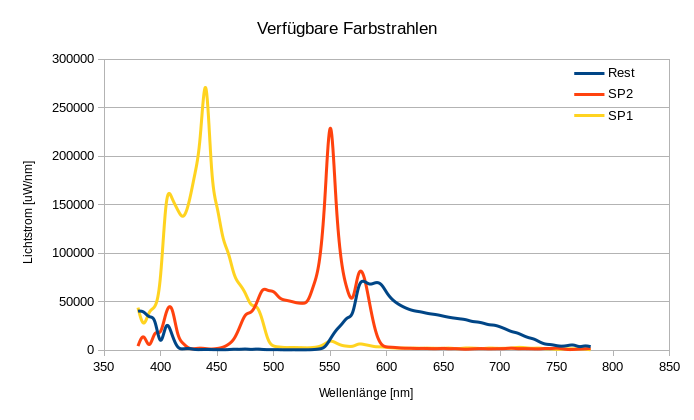
\includegraphics[scale=0.7]{Images/A_Farbstrahlen.png}
	\caption{Spektren der im Beamer aufgespalteten Farbstrahlen (Rot, Grün und Blau)}
\end{figure}
Für jede dieser Farbstrahlen wird nun die Farbkoordinate in der CIE-Normtafel berechnet. Hierfür wird, ausgehend von [\cite[Seite 26]{AML_SKRIPT}], das Spektrum jeder Farbe mit den drei Tristimuluskurven integriert. Die Tristimuluskurven in $5nm$-Schritten werden von [\cite[Seite 34]{AML_SKRIPT}] entnommen. Die Ergebnisse werden nun mit der Summe aller drei Ergebnisse normiert, und es ergeben sich die Koordinaten $x_n$ und $y_n$ wie folgt:

\begin{eqnarray*}
X_n = & \int\limits_{\mbox{380nm}}^{\mbox{780nm}} \Phi_{e\lambda,n}(\lambda)\cdot \overline{x}(\lambda)d\lambda \\
Y_n = & \int\limits_{\mbox{380nm}}^{\mbox{780nm}} \Phi_{e\lambda,n}(\lambda)\cdot \overline{y}(\lambda)d\lambda \\
Z_n = & \int\limits_{\mbox{380nm}}^{\mbox{780nm}} \Phi_{e\lambda,n}(\lambda)\cdot \overline{z}(\lambda)d\lambda \\
x_n = & \frac{X_n}{X_n+Y_n+Z_n} \\
y_n = & \frac{Y_n}{X_n+Y_n+Z_n}
\end{eqnarray*}
Da hier diskrete Werte in 5nm-Schritten für sowohl die Tristimuluskurven als auch die Lichtströme der Farbstrahlen vor liegen, kann hier nicht von Hand integriert werden. Stattdessen wird vereinfacht die Summe der wellenlängenspezifischen Multiplikation der Tristimuluskurve und Lichtstromes verwendet. Durch die hohe Anzahl der Schritte (N=80) ergibt sich ein relativ kleiner Fehler im Vergleich zu einer polynomialen Approximation. Da nach dem Ergebnis der Integrationen normiert wird, ist auch das $d\lambda$ vernachlässigbar. Es wird verwendet:
\begin{equation}
X_n = \sum_{i=0}^{80} \Phi_{e\lambda,n}(i*5nm + 380nm) \cdot \overline{x}(i*5nm + 380nm)
\label{A_SUM}
\end{equation}
Gleichung \ref{A_SUM} wird hier analog für $Y_n$ und $Z_n$ verwendet. In Tabelle \ref{A_COORDS} sind die berechneten Farbkoordinaten aufgelistet.

\begin{table}[h]
\caption{Berechnete erwartete Farbkoordinaten}
\centering
\begin{tabular}{| c | c | c | c | c | c |}
\hline
Strahl (n) & $X_n$ & $Y_n$ & $Z_n$ & $x_n$ & $y_n$ \\
\hline
Blau (1) & 585007 & 160445 & 2756357 & 0.1671 & 0.04582 \\
Grün (2) & 690939 & 1351575 & 316961 & 0.2928 & 0.57283 \\
Rot (3) & 803518 & 595402 & 26823 & 0.5636 & 0.4176 \\
\hline
\end{tabular}

\label{A_COORDS}
\end{table}
Der daraus resultierende theoretisch abbildbare Farbraum ist in Abschnitt \ref{A_FCOORDS}, Abbildung \ref{A_Farbdreieck} dargestellt. Er überschneidet sich zu 68\% mit dem sRGB-Farbraum, bzw. zu 49\% mit dem Adobe-RGB-Farbraum. Da das betrachtete Farbdreieck vollständig in den beiden Farbräumen liegt, wird diese Übereinstimmung durch Berechnung des relativen Flächeninhaltes kalkuliert. Dies ist für den betrachteten Beamer durchaus zu erwarten, da dieser aus Kostengründen mit hoher Wahrscheinlichkeit keine möglichst genaue Farbwiedergabe besitzten wird. Blau- und Grüntöne sind erwartungsgemäß weit außen, der Rotton jedoch ist relativ schwach ausgeprägt. Betrachtet man das Spektrum der Quecksilberdampflampe, so ist zu erkennen, dass die Lichtquelle selbst schon im Bereich des roten Lichtes weitaus weniger intensiv strahlt als in den grünen und blauen Wellenlängen.
\subsection{Auswertung und Vergleich}
\label{A_FCOORDS}

Im Anschluss an die Versuche und die Berechnungen der theoretischen und realen Farbspektren sollen diese von den Teilnehmenden nun miteinander verglichen werden. Hiermit wird der Bezug zwischen den aus den Messwerten berechneten theroetisch möglichen und dem realen Farbbereich hergestellt. Der real gemessene und der berechnete Farbbereich sind in Abbildung \ref{A_Farbdreieck} dargestellt.

\begin{figure}[h]
	\centering
	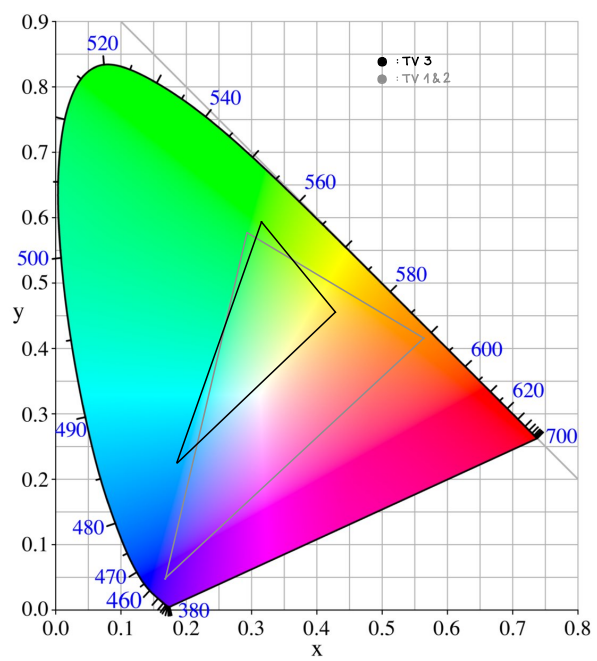
\includegraphics[scale=0.6]{Images/A_Farbdreieck.png}
	\caption{Berechneter und gemessener Farbraum des Beamers}
	\label{A_Farbdreieck}
\end{figure}

Sehr deutlich zu erkennen ist, dass der Farbraum des realen Beamers weitaus kleiner ist im Vergleich zum berechneten Erwartungswert. Der Anteil des grünen Lichtes (approximativ die y-Koordinate) des Lichtes ist auch bei voller Ansteuerung von Rot bzw. Blau immer höher in den Realwerten im Vergleich zu den in \ref{sec:Erwartungswerte} berechneten Erwartungswerten, lediglich der Grünkanal selbst ist bei Real- und Erwartungswerten nahezu gleich. Der reale Farbbereich überschneidet sich nur noch zu 19\% mit dem Adobe-Farbraum, bzw. zu 27\% mit dem sRGB-Farbraum, wenn mit der gleichen Methode der Flächeninhaltsberechnung wie in \ref{sec:Erwartungswerte} gearbeitet wird.

Begründet werden kann diese Verschlechterung durch eine Alterung der LCD-Elemente. Auch ohne Messungen konnten die Teilnehmer ein sehr grünliches Bild auch bei blauen und roten Bildern beobachten, d.h. die Rot- und Blaupunkte wurden stark beeinträchtigt. Zusätzlich wurden die Verluste an den dichroitischen Spiegeln nicht betrachtet, welche evtl. ein anderes Reflektionsspektrum als angenommen besitzen. Dies gilt auch für den Rekombinationsspiegel, welcher zusätzliche Verluste einbringt, und nicht berücksichtigt wurde. Auch sind Verluste an den LCD-Elementen selbst nicht betrachtet worden. All diese Verluste erklären gut die Abweichungen zwischen Real- und Erwartungswert, können hier jedoch nicht quantifiziert werden.

\subsubsection{Fazit}

In diesem Versuch konnten erfolgreich einige der Elemente eines handelsüblichen LCD-Beamers bemessen werden. Eine Berechnung des theoretisch möglichen Farbraumes war möglich, und lieferte plausible Werte. Die geringe Übereinstimmung mit dem realen Farbraum konnte ebenso erklärt werden durch eine Alterung des Beamers. Den Studierenden wurde somit ein Einblick in einige der wichtigen Elemente eines solchen Beamers geliefert, während weiter Fragestellungen wie z.B. der Einfluss der LCD-Schirme oder des Rekombinationsspiegels zu einer tieferen Auseinandersetzung mit dem Material geführt haben.

\newpage
\printbibliography

\end{document}